\section{Discrete Time Behavior} \label{sec:discrete_time_behavior}
So far, we've considered that the system is continuous time. 
This is a reasonable assumption, if we have a high sampling time $\Delta t$, compared to the dynamics, i.e., $\| \Delta t \, \dot{\vecs \xi} \| \ll 1$.
However, any digital controller sends a discrete control signal. In order to reject the disturbances in the presence of obstacles, a high control force is exerted (while still remaining within the control robot's limits), hence $\| \Delta t \, \vecs \tau^c \| \gg 1$. 
In this case, it is crucial to analyze the discrete-time system to guarantee stability, as high damping can lead to unstable behavior, see Figure~
\ref{fig:discrete_controller_parameters_comparison}).

\begin{figure}[htb]
\centering
  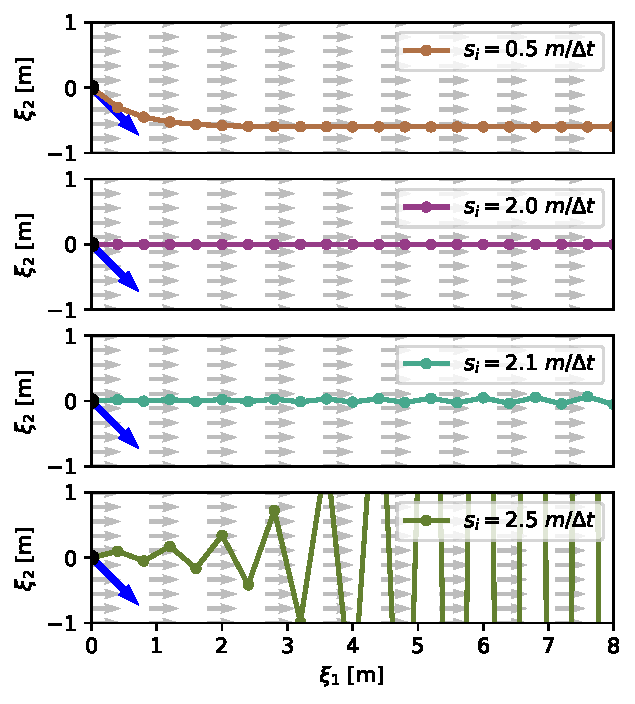
\includegraphics[width=\columnwidth]{figures/discrete_controller_parameters_comparison}
  \caption{A point-like agent with an initial velocity of $\{ \dot{\vecs \xi} \}_0 = [1 \; -1]^T$ is guided by the desired velocity $\vect f(\vecs \xi) = [1, 0]^T$, and a control matrix $\matd{D}$ with damping values $s_i$ equal in all directions, where $m$ is the mass of the point-like agent. 
  Damping values above $s_i = 2.0 m / \Delta t$ lead to unstable behavior where the higher value leads to higher oscillations. Conversely, the lowest value leads to more deviation from the straight trajectory resulting from the higher impedance. The critical value of $s_i = 2.0 m / \Delta t$ results in stable behavior with immediate correction to the desired velocity.}
  \label{fig:discrete_controller_parameters_comparison}
\end{figure}

For the discrete-time system, the position and velocity of the agent evolve as follows:
\begin{equation}
	\begin{bmatrix}
	 \vecs \xi_{t+1} \\ \dot{\vecs \xi}_{t+1}
	\end{bmatrix}
	=
	\begin{bmatrix}
	 \vecs \xi_{t} \\ \dot{\vecs \xi}_{t}
	\end{bmatrix}
	+ 
	\Delta t 
	\begin{bmatrix}
		\dot{\vecs \xi}_{t} \\ \ddot{\vecs \xi}_t 
	\end{bmatrix}
	\label{eq:discrete_time_dynamics}
\end{equation}

\begin{lemma}
	Let us consider a discrete-time system given in \eqref{eq:discrete_time_dynamics}, which is governed by the controller \eqref{eq:control_command} and damping matrix $\matd{D}$ defined in \eqref{eq:damping_summation}.
	Let us consider the input the desired velocity $\vect f(\vecs \xi)$ and as output the agent's velocity $\dot{\vecs \xi}$. 
	The system is BIBO (bounded-input, bounded-stable) with respect to the velocity, i.e., $\lim_{t \rightarrow \infty} \| \dot{\vect \xi} \| < \infty$, if all eigenvalues of $\matd{M}^{-1} \matd{D}$ are less or equal to $2 / \Delta t$.
\end{lemma}

\begin{proof}
Hence, for the evaluation in discrete time, the evolution of the velocity is given by:
\begin{equation}
	\begin{split}
	& \begin{bmatrix}
	 \vecs \xi_{t+1} \\ \dot{\vecs \xi}_{t+1}
	\end{bmatrix}
	=
	\begin{bmatrix}
		\vect \xi_t + \Delta t  \; \dot{\vect \xi}_t \\ \
		\dot{\vecs \xi}_t + \Delta t \, \matd{M}^{-1} \left( \matd{D}(\vect \xi_t) \left( \vect f(\vecs \xi_t) - \dot{\vecs \xi}_t \right) - \matr C \right)
	\end{bmatrix} \\
	&  = %\approx
	\begin{bmatrix}
		1 & \Delta t \\
		0 & 1 - \Delta t \matd{M}^{-1} \matd D 
	\end{bmatrix}
	\begin{bmatrix}
		\vect \xi_t \\ \dot{\vect \xi}_t
	\end{bmatrix}
	+ \begin{bmatrix}
		0 \\ 
		\Delta t \, \matd{M}^{-1} \matd{D} 
	\end{bmatrix}
	\hat{\vect f}(\vecs \xi_t) 
	% & \approx 
	% \begin{bmatrix}
	% 	1 & \Delta t \\
	% 	\Delta t \matd{M}^{-1} \matd D \frac{\partial \vect f}{\partial \vecs \xi} & 1 - \Delta t \matd{M}^{-1} \matd D 
	% \end{bmatrix}
	% \begin{bmatrix}
	% 	\vect \xi_t \\ \dot{\vect \xi}_t
	% \end{bmatrix}
	\label{eq:discrete_time_proof}
	\end{split}
\end{equation}
where $\hat{\vect f}(\vecs \xi_t) = \vect f(\vecs \xi_t) - \matd{D}^{-1} C$. 
As we look at global stability, the Coriolis acceleration $\matd{C}$ is merged into the dynamical system. Since the Coriolis force is bounded, it follows that if the system is BIBO stable for $\hat{\vect f}(\vect \xi)$ then it is also BIBO stable for $\vect f(\vecs \xi)$ 

% Let us introduce the coordinate transform $\dot{\vect \gamma}_t = \dot{\vect \xi}_t - \vect f(\vecs \xi)$  and hence for the position we have $\vect \gamma_t = \vect \xi_t - \Delta t \vect f(\vecs \xi)$, and hence 
% \begin{equation}
% 	\begin{split}
% 		\begin{bmatrix}
% 			\vect \gamma_{t+1} \\ \dot{\vect \gamma}_{t+1}
% 						\end{bmatrix}
% 	& =	
% 	\begin{bmatrix}
% 		1 & \Delta t \\
% 		0 & 1 - \Delta t \, \matd{M}^{-1} \matd{D}
% 	\end{bmatrix}
% 	\begin{bmatrix}
% 		\vecs \gamma_t \\ \dot{\vecs \gamma}_t
% 	\end{bmatrix}
% 	+ \begin{bmatrix} 
% 	\Delta t \vect f(\vecs \xi_t) \\ 0
%     \end{bmatrix} \\
% 	& \approx \begin{bmatrix}
% 		1 + \Delta t \frac{\partial \vect f}{\partial \vect \xi} & \Delta t \\
% 		0 & 1 - \Delta t \, \matd{M}^{-1} \matd{D}
% 	\end{bmatrix}
% 	\end{split}
% \end{equation}
% The summand $\vect t \vect f(\vecs \xi_t)$ changes the relative position value $\vect \gamma_t$ as long as the desired velocity is not zero. However, this only moves the relative position but does not influence kinetic energy, which has been used as the stability function (Section~\ref{sec:passivity_analysis}).

BIBO stability of a discrete-time system requires that all the eigenvalues of the feedback matrix are smaller or equal to one.
The eigenvalues of the above feedback matrix are given as:
\begin{equation}
	\vect \lambda_1 = 1 \qquad \vect \lambda_2 = 1 - \Delta t \, \matd{M}^{-1} \matd{D}
\end{equation}
The first eigenvalue is stable by design; the second feedback eigenvalue is stable if the maximum eigenvalue of the matrix. 
Hence, the system is stable if the eigenvalues are smaller or equal to one \cite{friedland2012control}. This is the case if the maximum of $\matd{M}^{-1} \matd{D}$ is larger or equal to $\leq 2 / \Delta t$.
\end{proof}


\subsection{Asymptotic Stability}
The stability guarantees in the previous section; the system's stability was reduced to boundedness. 
Since the first eigenvalue equals one, asymptotic convergence does not occur. 
This implies that if the input goes to zero, i.e., $\vect f(\vecs \xi) = \vect 0$, the system stops and does not converge to a specified point. Since the desired velocity should only reach zero at the attractor, the system is expected to converge in most cases.

Yet, asymptotic stability is not guaranteed for general nonlinear input dynamics. Especially for dynamics with high curvature and low damping value, the final trajectory can end up in limit cycles ((Figure~\ref{fig:discrete_controller_parameters_comparison_stable}).

\begin{figure}[htb]
\centering
  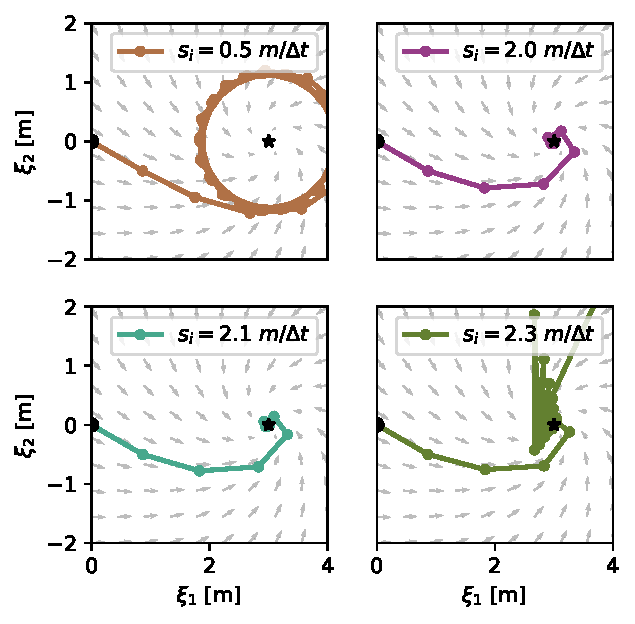
\includegraphics[width=\columnwidth]{figures/discrete_controller_parameters_comparison_stable}
\caption{A point-like agent which is following the desired dynamics of
$\vect f(\vecs \xi) = \matr R(\pi / 6) (\vect \xi  - \vect \xi^a)$ where $\matr R(\cdot)$ is the rotation matrix, and with equal damping values $s_i$, where $m$ is the mass of the agent.
The controller with a critical stiffness of $2.0 m / \Delta t$ leads to fast convergence and a stable system. With lower damping (top left), there is a large drift of the system and the system converges to a limit cycle. 
The high damping of $2.3 m / \Delta t$ leads to an unstable system. 
Interestingly, with stiffness of $2.1 m / \Delta t$ in combination, we obtain a visibly stable system.}
  \label{fig:discrete_controller_parameters_comparison_stable}
\end{figure}

% For a general nonlinear system no asymptotic convergence evaluation can be made. This is due to the fact, that for any system there is a slight drift due to the damping values.
% And hence, if there are high nonlinearities in the system it could happen that even with a stable system, the dynamics get caught in a limit cycle. However, for most common globally asymptotic systems (for velocity-position), the force controller as proposed leads to globally asymptotically stable behavior, too (Figure~\ref{fig:discrete_controller_parameters_comparison_stable}).

% \subsection{Intertial Drift}
% Let us assume that have strong damping in the direction of the obstacle, i.e., $s^{\mathrm{obs}} / m_i \gg 1$, where $m_i$ with $i = 1, .., N$ represent the eigenvalues of the mass matrix $\matd{M}$. 
% 
